\documentclass[10pt,journal,compsoc]{IEEEtran}



% *** CITATION PACKAGES ***
%
\ifCLASSOPTIONcompsoc
  % The IEEE Computer Society needs nocompress option
  % requires cite.sty v4.0 or later (November 2003)
  \usepackage[nocompress]{cite}
\else
  % normal IEEE
  \usepackage{cite}
\fi

% *** GRAPHICS RELATED PACKAGES ***
%
\ifCLASSINFOpdf
 
\else
  
\fi

\ifCLASSOPTIONcompsoc \usepackage[caption=false,font=normalsize,labelfon
t=sf,textfont=sf]{subfig}
\else
\usepackage[caption=false,font=footnotesize]{subfi g}
\fi


\usepackage{graphicx}
\usepackage{algorithmic}
\usepackage{algorithm}
\renewcommand{\algorithmicrequire}{\textbf{Input:}} 
\renewcommand{\algorithmicensure}{\textbf{Output:}}
%\usepackage{cases}
\usepackage{amsmath}
\usepackage[overload]{empheq}
\newcommand{\for}{\text{for }}

\newcommand\MYhyperrefoptions{bookmarks=true,bookmarksnumbered=true,
pdfpagemode={UseOutlines},plainpages=false,pdfpagelabels=true,
colorlinks=true,linkcolor={black},citecolor={black},urlcolor={black},
pdftitle={Bare Demo of IEEEtran.cls for Computer Society Journals},%<!CHANGE!
pdfsubject={Typesetting},%<!CHANGE!
pdfauthor={Michael D. Shell},%<!CHANGE!
pdfkeywords={Computer Society, IEEEtran, journal, LaTeX, paper,
             template}}%<^!CHANGE!

\hyphenation{op-tical net-works semi-conduc-tor}

\begin{document}

\title{QoS-Oriented Mobile Service Composition Over Oppotunistic Networks}

\author{Qinglan~Peng,~\IEEEmembership{Member,~IEEE,}
        John~Doe,~\IEEEmembership{Fellow,~OSA,}
        and~Jane~Doe,~\IEEEmembership{Life~Fellow,~IEEE}% <-this % stops a space
\IEEEcompsocitemizethanks{\IEEEcompsocthanksitem M. Shell was with the Department
of Electrical and Computer Engineering, Georgia Institute of Technology, Atlanta,
GA, 30332.\protect\\
% note need leading \protect in front of \\ to get a newline within \thanks as
% \\ is fragile and will error, could use \hfil\break instead.
E-mail: see http://www.michaelshell.org/contact.html
\IEEEcompsocthanksitem J. Doe and J. Doe are with Anonymous University.}% <-this % stops a space
\thanks{Manuscript received April 19, 2005; revised August 26, 2015.}}



% The paper headers
\markboth{Journal of \LaTeX\ Class Files,~Vol.~14, No.~8, August~2015}%
{Shell \MakeLowercase{\textit{et al.}}: Bare Advanced Demo of IEEEtran.cls for IEEE Computer Society Journals}

\IEEEtitleabstractindextext{%
\begin{abstract}
The abstract goes here.
\end{abstract}

% Note that keywords are not normally used for peerreview papers.
\begin{IEEEkeywords}
Computer Society, IEEE, IEEEtran, journal, \LaTeX, paper, template.
\end{IEEEkeywords}}


% make the title area
\maketitle



\IEEEdisplaynontitleabstractindextext

\IEEEpeerreviewmaketitle


\ifCLASSOPTIONcompsoc
\IEEEraisesectionheading{\section{Introduction}\label{sec:introduction}}
\else
\section{Introduction}
\label{sec:introduction}
\fi


\IEEEPARstart{R}{ecent years} have witnessed the rapid development of mobile devices and mobile communication technology, mobile devices has already surpassed stationary Internet hosts in numbers and web services are no longer limited to traditional stationary platforms and they can be more flexible and pervasive. The hardware of mobile devices will continue to make breakthroughs on extending the capabilities of mobile devices in terms of computational power, RAM, storage capacity, and so on \cite{Deng2017}. The huge potential of mobile technology brings a great opportunity to traditional service computing in the mobile environment. As a result, the global interest of mobile service is on the rise and both academia and industry are inspired to pave the way for mobile service provisioning \cite{dinh2013survey,hu2014multidimensional}.

While mobile device have powerful computing and communication capabilities now, the resources-intensive services, however, drain out the energy of the device much faster than before. 
To achieve the goal of reducing mobile device energy consumption, we propose a QoS-oriented mobile service composition approach in this paper, where a mobile user in mobile opportunistic network can combine and exploit nearby devices' resources to boost their computing power and overcome the limitations of their own resources. As shown in fig.1, this architecture can reduce communication energy consumption and avoid the extreme centralization of traditional mobile cloud computing \cite{Giordano2011}. Its main rationality is three-fold. First, opportunistic user encounters are prevalent and sufficient in daily life \cite{liu2013exploring}, which offers plenty of opportunities to exploit nearby mobile worker for task solving \cite{chang2015progressive,heimerl2012communitysourcing,agapie2015crowdsourcing}. Second, many mobile tasks require huge computational resources or data transfer (e.g., Tensorflow on mobile, Photoshop on mobile, Online video), for energy consumption and cost perspective, nearby mobile service provider are more adept at executing these tasks than the online workers, because this paradigm can reduce data transfer over cellular network which consume more energy than device to device (D2D) communications such as Bluetooth, WiFi and NFC \cite{Balani}. Third, D2D communications are promising to replenish traditional cellular communications in terms of user throughput increase, cellular traffic reduction and network coverage extension, in this way, users can get better quality of service and save communication fee\cite{asadi2014survey}. In a word, this framework shares the similar spirit with the emerging paradigm “cyber foraging” over opportunistic networks, such that mobile users opportunistically exploit nearby device resources to facilitate their computational task processing \cite{shi2012serendipity,li2014can,zhang2015offloading}.

\begin{figure}[!t]
\centering
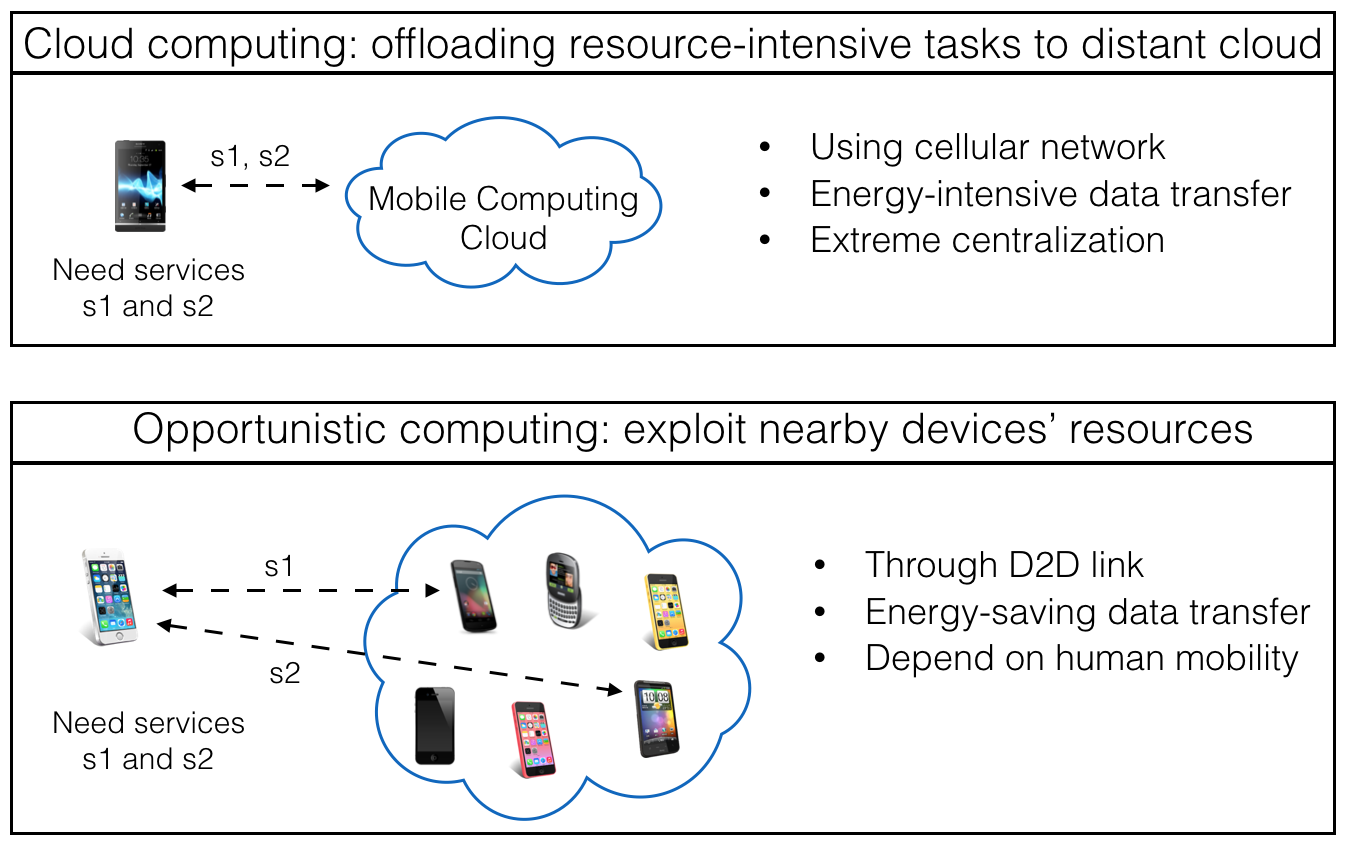
\includegraphics[width=3.5in]{./img/pic1.png}
\caption{Opportunistic computing}
\label{fig_opportunistic}
\end{figure}

To address the aforementioned challenges and concerns, we propose a new approach for mobile service composition over opportunistic network. The main contributions are:

1) We propose a framework (mobile service opportunistic network MSON) to address the problem of service provision in the mobile encounter environment where both service requesters and providers are nonstationary. In such environment, mobile user can invoke service exposed by nearby mobile devices through D2D links.

2) For MSON, we propose a mobile service QoS model for service provision which consider mobile service availability as an important QoS attribute to capture user's mobility behavior.

3) Based on MSON and the proposed mobile service QoS model, we transfer the mobile service composition problem to an optimization problem and use the Krill-Herd algorithm (KH) to solve it. A series of evaluations have been conduct to validate the optimality and scalability of our algorithm, and it shows our algorithm can get approximately optimal solution and better performance than other standard composition approaches. 

The remainder of this paper is structured as follows. Section II describe the MSON framework and its application scenario. Section III introduces the mobile service composition model. The approach to make service compositions is presented in Section IV. Section V presents experiments and evaluations. Section VI reviews the related work. Section VI concludes this paper.

\section{MSON AND APPLICATION SCENARIO}

\begin{figure}[!t]
\centering
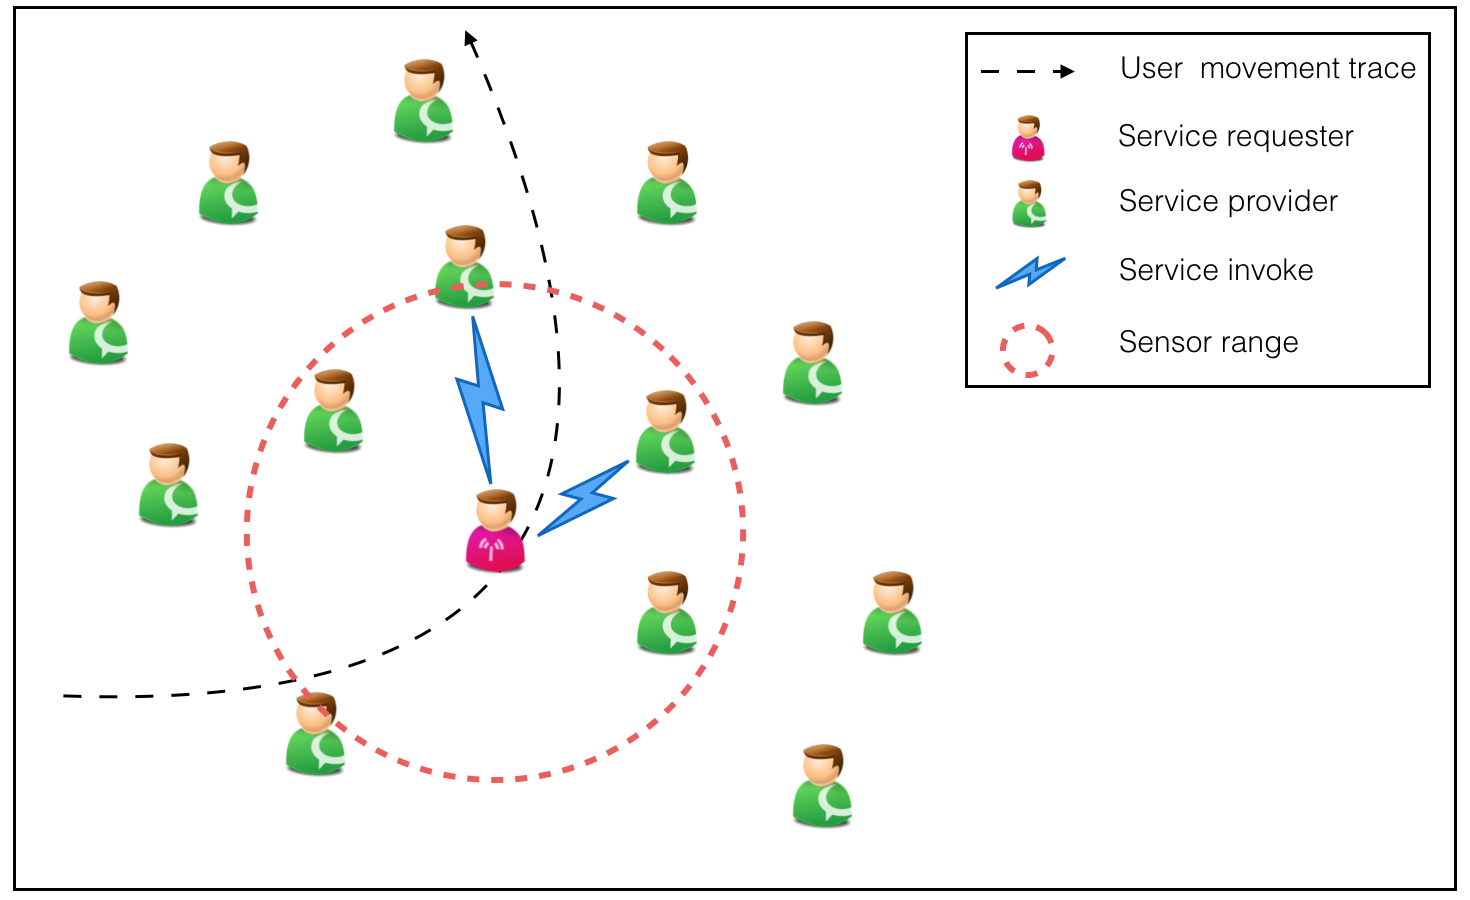
\includegraphics[width=3.5in]{./img/pic2.png}
\caption{Mobile service opportunistic network}
\label{fig_mson}
\end{figure}

In this section, we first introduce the characteristics mobile service opportunistic network (MSON), then an example is presented to illustrate its application scenario.

MSON has three main characteristics:

1) Locality: An MSON is not established through the stable Internet, it do not consider user mobility a problem but as an opportunity to exploit. Mobile user in opportunistic network can discover nearby service and establish self-organized local communication network within sensor distance.

2) Mobility: Services requesters and providers are not fixed at the same location, and they are mobile when invoking or provisioning a mobile service.

3) Nondeterminacy: MSON participants are not stationary, one node can enter or leave the data transmission range of other nodes at any time. 

Fig.2 illustrates the working procedure of the mobile service provision over opportunistic network. In an opportunistic network scenario, a mobile service requester $R$ can discover mobile service exposed by nearby devices through D2D link and launch a mobile composition request. A composer can be implemented and deployed on the requester's mobile device, which is in charge of discovering available mobile services nearby, selecting appropriate concrete service, and composing multiple services. During the execution of mobile service compositions, all concrete services interact with the composer directly \cite{Deng2017}.

Note that, our framework only considers one-hop mechanism for both service requester and provider, since some realistic dataset analyses reveal that users' one-hop neighbors are sufficient, compared with multi-hop mechanisms in existing researches \cite{chang2015progressive,karaliopoulos2015user,han2016competition,tuncay2013participant,wu2013homing,jiang2016exploiting,liu2013exploring}, D2D communication which hops are larger than two would incur long delay \cite{li2014can},  this one-hop feature can lower the network overhead (e.g., no need to transfer a large volume of task contents hop by hop) and ensure framework choose only local relatively reliable service. 

We use an example to illustrate the related features of service provision over MSON. Assume a mobile user Mike just complete his tour and now he is on the subway to airport. Now he wants to edit some videos he recorded and add some effects and share these video clips with his friends. But due to mobile devices' limited battery, if he edit videos in his own mobile device, his mobile phone will run out of energy before he reach the destination. As one option, he can upload original videos to cloud and use cloud service to get all things done, but offloading quest into cloud will result in heavy cellular traffic, that means expensive communication fee and high energy consumption. If Mike participate in MSON and several video processing services is provided by some nearby mobile devices, Mike can invoke such mobile services on nearby mobile devices through D2D communication techniques. If these services cannot meet his requirement, several services can be composed. Due to users' mobility, the availability of service to Mike can vary, invoking mobile services provided by other users may face new challenges that traditional composition methods cannot handle. Thus, a mobile service composition model which can capture mobile services' availability need to be proposed, we will discuss mobile service availability in next section \cite{Deng2016-2}.


\section{MOBILE SERVICE COMPOSITION MODEL}
In this section, we first give some basic concepts of mobile service composition, then introduce the concept of mobile service availability, finally we propose a specific QoS model for mobile service composition over opportunistic network.
\subsection{Preliminaries}
In order to describe the problem addressed in this paper, we first provide the basic concepts of mobile service composition.

\textit{Definition 1 (Mobile Service):} A mobile service can be represented as a three-triple $ms = (id, info, QoS)$, where:

​1) $id$ is the unique identifier of the service;

2) $info$ is the description of a mobile service which include service name, functionality, parameters and result.

​3) $QoS = \{q\}^n_{j=1}$ is a set of quality attributes, including response time, price, availability, etc.

\textit{Definition 2 (MSON participant):} A MSON participant is mobile service user who can be both service provider and requesters, it can be represented by a three-tuple $u = (id, P, C)$, where:

​1) $id$ is the unique identifier of a MSON participant;

​2) $p$ is the set of mobile services exposed by mobile service user $u$.

​3) $c$ is the set of discovered mobile services from nearby mobile service providers.

\textit{Definition 3 (Mobile Service Composition Plan):} A service composition plan is a tuple $mscp = (T, R)$, where:

​1) $T = \{t_1,t_2,…,t_n\}$ is a set of tasks;

​2) $R = \{d(t_i,t_j)|t_i,t_j \in T\}$ is a set of relations between tasks in $T$.

​A service composition plan is an abstract description of a business process. Each task $t_i$ can be realized by invoking an individual service. $R$ is used to describe the structure of the composition. $d(t_i, t_j) = 1$ represents that the inputs of $t_j$ depend on the outputs of $t_i$.

\textit{Definition 4 (composite service instance):} A service composition instance is a tuple $csi = (mscp, S)$, where:

​1) $mscp$ is mobile service composition plan which defined in definition 3;

​2) $S = {s_1, s_2,…,s_n}$ is a set of selected concrete services.

\subsection{Concept of Mobile Service Availability}
In mobile service opportunistic network (MSON) the availability of mobile service is highly related to the user’s mobility. If user $i$ moves outside the transmission range of its neighbouring user $j$, then user $i$ is unreachable by user $j$ and as a result the services on user $i$ become unavailable to user $j$ either. Here user mobility is utilized to calculate the mobile service availability \cite{Yang2010}.

\textit{Definition 5 (Mobile Service Availability):} mobile service availability can be represented by a three-tuple $(i, p, ava) $, where

​1) $r$ is the mobile service requester;

​2) $p$ is the mobile service provider;

​3) $ava$ is the mobile service availability value between requester $r$ and provider $p$, $ava \in [0,1)$, and $ava=0$ means service provider $p$ moves out of transmission range.


\begin{figure}[!t]
\centering
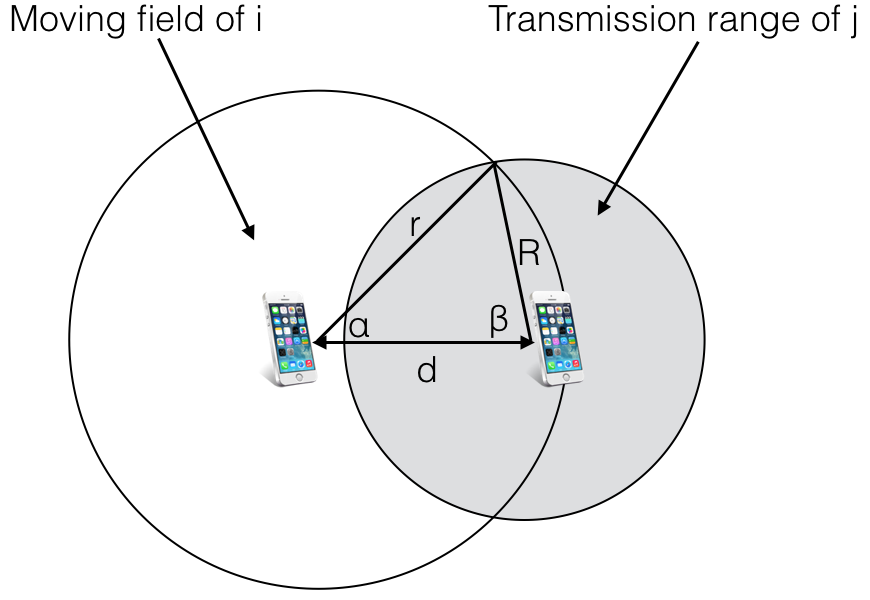
\includegraphics[width=3.5in]{./img/pic3.png}
\caption{Mobile service availability}
\label{fig_sd}
\end{figure}

As illustrated in Fig.3, there are two mobile user $i$ and $j$ whose device have the same transmission range $R$. Each user moves randomly and it is assumed that the moving field is a circle with a radius of $r$. $d$ is the distance between $i$ and $j$. We use these three parameters($r,R,d$) to calculate the availability of a mobile service. The transmission range of a node $R$ is known (e.g., pre-defined or changing according to certain algorithm). Suppose that the location of each mobile user is known (e.g., via GPS data or other location-based services provided by telecommunications service providers \cite{chadil2008real}), then distance $d$ can be calculated using the Euclidean distance formula, i.e.,$\sqrt{{(x_i-x_j)^2}+({y_i-y_j})^2}$ where $(x_i, x_j)$ and $(y_i, y_j)$ are the coordinates of user $i$ and $j$ respectively. Finally let us discuss how to calculate $r$ \cite{Yang2010}.

The moving radius of a mobile user $r$ is its moving speed $v$ multiplied by the average service time $t$. Here $t$ can be statistically calculated as the average value of last $n$ times of service invoke, namely, $t = \Sigma_{i=1}^{n}t_i/n$. The speed of a mobile user $v$ can be calculated based on its moving distance during a period from $t_1$ to $t_2$ \cite{ko2000location}, namely: $s = \sqrt{{(x_i-x_j)^2}+{y_i-y_j}^2}/(t_2-t_1)$, then $r = s \times t$.

​Once we know these three parameters $R$, $r$, and $d$, the probability of user $i$ staying inside the transmission range of user $j$ (denoted as $P_{i,j}^{IN}$ ) can be calculated by
\begin{equation}
P_{i,j}^{IN} = \frac{S_i^{IN}}{S_i^T}
\end{equation}
Namely, $P^{IN}_{i,j}$ equals to the area of the user $i$ moving field inside the transmission range of user $j$ (denoted as $S^{IN}_i$) divided by the overall area of the user $i$ moving field ($S^T_i$) .
\begin{eqnarray}
\alpha = arccos(\frac{r^2+d^2-R^2}{2r\times d}) \\\nonumber
\beta = arccos(\frac{R^2+d^2-r^2}{2r\times d})
\end{eqnarray}
Then,
\setlength{\arraycolsep}{0.0em}
\begin{eqnarray}
S^{IN}_i&{}={} &[(\frac{2\beta}{2\pi}\pi R^2)-(\frac{R sin\beta cos\beta}{2}2)]\\\nonumber
&&+ [(\frac{2\alpha}{2\pi}\pi r^2)-(\frac{r sin\alpha cos\alpha}{2}2)]\\\nonumber
&&= \beta R^2 + \alpha r^2 - (R^2 sin\beta cos\beta + r^2 sin\alpha cos\alpha)
\end{eqnarray}
\setlength{\arraycolsep}{5pt}
There is also
\begin{equation}
S_i^T = \pi r^2 = \pi \times (s \times t)^2
\end{equation}
Therefore, the probability of user $i$ staying inside the transmission range of user $j$, $(P^{IN}_{i,j})$, can be calculated as follow
\begin{equation}
P_{i,j}^{IN} = \frac{S_i^{IN}}{\pi s^2 t^2}
\end{equation}
Suppose a mobile service $s$ running on $i$ is a candidate service for a task requested by user $j$, and the availability of candidate service $s$ can be denoted as $q_{ava}(s)$, that is
\begin{eqnarray}
q_{ava}(s) &{} = {}& P^{IN}_i \\\nonumber
&& = \frac{A_i^{IN}}{\pi s^2 t^2}\\\nonumber
&& = \frac{\beta R^2 + \alpha r^2 - (R^2 sin\beta cos\beta + r^2 sin\alpha cos\alpha)}{\pi s^2 t^2}
\end{eqnarray}
Mobile service availability $q_{ava}(s)$ can capture user's mobile behavior, and we use it as an important QoS attribute to construct QoS model for service composition in next subsection.

\subsection{QoS Model for Mobile Service Composition}
For mobile service requesters to select candidate service, QoS must be considered \cite{wu2013predicting,luo2014efficient,luo2016generating}. Generally, QoS attributes include response time, price, reliability, and reputation, we introduce mobile service availability as an important QoS attribute in this paper to describe user's mobility behavior. QoS attributes in this paper can be classified into two categories: positive ($Q^+$) and negative ($Q^{-}$). For positive attributes, larger values indicate better performance (e.g., reputation and availability), while for negative attributes, smaller values indicate better performance (e.g., response time and cost) \cite{Wu2016}.	

\begin{table}[!t]
\renewcommand{\arraystretch}{1.3}
\caption{EXAMPLES OF AGGREGATION FUNCTIONS FOR QOS}
\label{table_example}
\centering
\begin{tabular}{ccc}
\hline
\bfseries Pattern & \bfseries Resopnse Time & \bfseries Availability \\
\hline
sequence & $\sum_{i=1}^{n}q_{time}(S_i)$ & $\sum_{i=1}^{n}q_{price}(S_i)$ \\
parallel & $Max\{q_{time}(S_i)\}$ & $\sum_{i=1}^{n}q_{price}(S_i)$ \\
choice & $\sum_{j=1}^{n} p_j \times q_{time}(S_j)$ & $\sum_{j=1}^{n} p_j \times q_{price}(S_j)$ \\
loop & $k \times q_{time}(S_i)$ & $k \times q_{price}(S_i)$ \\
\hline
\end{tabular}
\end{table}

For a composite service instance $csi$, its each QoS attribute is determined by its concrete components and orchestration patterns. Table.1 lists the aggregation functions for response time, cost, and availability for sequential, loop, choice, and parallel composition patterns. We can find more aggregation functions found in \cite{jaeger2004qos} and \cite{zheng2013qos}.

In order to facilitate ranking of different composite service instances $csi$ in terms of QoS, we utilize simple additive weighting (SAW) as the QoS utility function to map the QoS value into a real value. SAW first normalizes the QoS attribute values into real values between $0$ and $1$, through comparison with the maximal and minimal values; then it sums the normalized values multiplied with a preference weight $w_t$. According to SAW, the QoS utility of a $csi$ can be calculated using e.q (7), where, $q_t(csi)$ is the aggregated value of the $t$-th QoS attribute of $csi$, and $q_{t,max}$ and $q_{t,min}$, respectively, denote the maximal and minimal possible aggregated values of the $t$-th QoS attribute \cite{Wu2016}.
\begin{eqnarray}
U(csi) = \sum_{q_t \in Q^-} \frac{q_{t,max}-q_t(csi)}{q_{t,max}-q_{t,min}}\times w_t \\\nonumber
+\sum_{q_t \in Q^+} \frac{q_t(csi)-q_{t,max}}{q_{t,max}-q_{t,min}}\times w_t
\end{eqnarray}

\subsection{Problem Formulation}
Base on the above discussion, we can give the definition of the service composition over MSON problem.
\textit{Definition 6 (MSON Service Composition):} Given a service composition request $req$ by a mobile user $u$, perceive nearby service and select suitable concrete services provided to achieve an optimal service composition instance $csi$ with the best QoS, that is
\begin{eqnarray}
target \ : \  max \ U(csi)\qquad\  \\\nonumber
subject \ to: \ i \in \{1,2,3,...,n \}  \\\nonumber
x_i \in \{1,2,3,...,m \}
\end{eqnarray}
where $U(csi)$ is the objection mentioned in e.q (7), $i \in [1,n]$ is the index of the tasks in the composition plan, $x_i \in [1, m]$ is the index of service candidates for the $i$-th task.

\textit{Theorem 1:} The service composition problem over MSON (Definition 6) is NP-hard.

\textit{Proof:} We can reduce our studied problem to a knapsack problem, and this problem can be solved by integer programming. The standard integer program to find the smallest value of a given objective function $F( \Theta)$ with a feasible parameter follows \cite{glover1986future}:
\begin{eqnarray}
inf \ F(\Theta) \qquad \qquad \quad \\\nonumber
subject \ to: \ \theta_i \in\{1,2,3,...,N\}
\end{eqnarray}

For the problem of selecting optimal services composition over MSON, the vector $\Theta= (\theta_1, . . . , \theta_n)$ can describe a possible solution as a service composition with $n$ tasks. An element $\theta_i$ in corresponds to a selected service from the candidates for the $i$-th task. The optimal solution  $\Theta*$ satisfies the following conditions:

1) $\Theta *$ belongs to the feasible set.

​2) $\forall \Theta, F(\Theta*) \le F(\Theta)$. 

The target of the mobile service composition problem in MSON is to find to obtain the biggest $F( \Theta)$. Thus, the problem is equivalent to the integer programming problem which is known to be NP-hard. Then the service composition problem over MSON is NP-hard.

\section{Composition Algorithm}
For the problem we formulate above, integer programming can be utilized to obtain the optimal solution. However, integer programming might cost much more time with the increment of problem size because of its poor scalability \cite{nemhauser1988integer}. To solve this problem in polynomial time, an meta-heuristic algorithms such as GAs and PSO, can be utilized to find the near optimal solution.
In this section, we will illustrate our algorithm for making mobile service compositions over MSON based on the Krill-Herd algorithm.

​KH algorithm \cite{gandomi2012krill} is new generic stochastic optimization approach for the global optimization problem which is inspired by predatory behavior and communication behavior of krill. 
In this paper, the position vector of each krill individual corresponds to a feasible mobile service composition, 
the foraging motion is to learn from the current optimal service composition. 
Similarly, the motion induced by other krill individuals means to learn from neighbor mobile service compositions.
The krill individual with the best position corresponds to the optimal mobile service composition. 
The KH optimization's target is to find the krill individual with the best position, which means to find the best mobile service composition with the best fitness value. 
Therefore, once the optimal krill individual is found, the best mobile service composition is obtained.

As shown in equation (10), the position of a krill individual is determined by three main factors: 1) foraging action; 2) movement influenced by other krill; and 3) physical diffusion. 
\begin{equation}
\frac{dcsi_i}{dt} =N_i+F_i+D_i
\end{equation}

where $csi_i = (s_{i,1}, s_{i,2}, . . . , s_{i,n})$ is $i$-th composition service instance ($csi$), $n$ is the number of tasks in the service composition, $s_{i,j}$ is the selected candidate for the $j$-th task in solution $csi_i$, where $N_i$, $F_i$, and $D_i$ denote the motion influenced by other $csi$, the foraging motion, and the physical diffusion of the $csi_i$, respectively.

1) Movement induced by other krill individuals

Motion induced by other composition service instance $N_i$ can be formulated as follow
\begin{equation}
N^{new}_i = N^{max}\alpha_i + \omega_n N^{old}_i
\end{equation}

where
\begin{equation}
\alpha_i = \alpha^{local}+\alpha^{target}
\end{equation}

$\alpha_i$ is direction of the induced motion and it can be evaluated by target swarm density (target effect $\alpha^{target}$), local swarm density (local effect $\alpha^{local}$). $N^{max}$ is the maximum induced speed, $\omega_n \in [0, 1]$ the inertia weight of the induced motion, $N^{old}_{i}$ is the last induced motion influenced by other $csi$.

2) Foraging Motion

Foraging Motion $F_i$ covered two parts: the current food location and the information about the previous location. For the $csi$ i, we formulated this motion below:

\begin{equation}
F_i = V_f\beta_i + \omega_f F^{old}_i
\end{equation}

where

\begin{equation}
\beta_i = \beta_i^{food}+\beta_i^{best}
\end{equation}

where $V_f$ is the foraging speed (empirically set to $0.02$ in this paper), $\omega_f∈ [0, 1]$ is the inertia weight of foraging, and $F^{old}_i$ is the last foraging motion. $\beta_i$ is the direction of the foraging motion.

3) Random diffusion

For the $i$-th $csi$, the physical diffusion is considered to be a random process. This motion includes two components: a maximum diffusion speed and a random directional vector, it can be formulated as follows

\begin{equation}
D_i = D^{max}\delta
\end{equation}

where $D^{max}$ is the maximum diffusion speed and $\delta \in [-1, 1]$ is a random directional vector. In this paper, the maximum diffusion speed is randomly generated in $[0.002, 0.01]$. 

4) Crossover operator

\begin{figure}[!t]
\centering
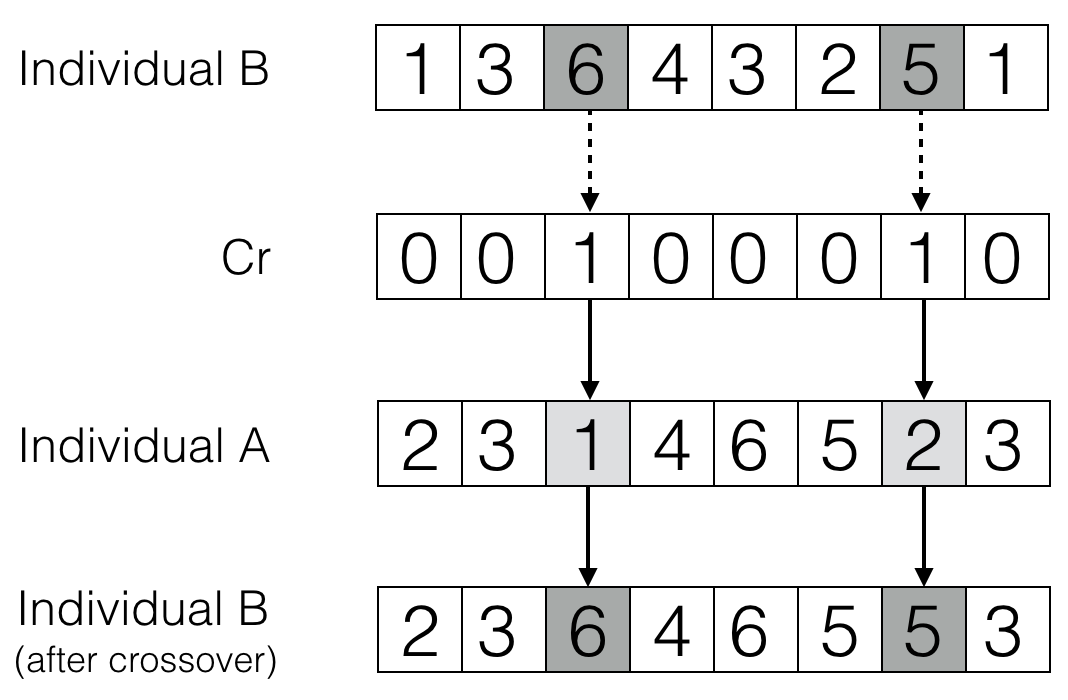
\includegraphics[width=2.5in]{./img/pic4.png}
\caption{Cross over}
\label{fig_opportunistic}
\end{figure}


The crossover operator plays an important role in Genetic algorithm for global optimization, we use this operator in KH algorithm to enhance the search capability. The crossover operator in this paper is controlled by crossover rate $C_{rate}$ which can be obtain as follow:
\begin{equation}
C_{rate} = 0.8 + 0.2 \times \frac{F_{best}-F_{i}}{F_{best}-F_{worst}}
\end{equation}

Where $C_{rate}$ is the $i$-th individual's crossover rate, $F_{i}$ is the $i$-th individual's fitness value, $F_{best}$ is the best fitness value so far, similarly, $F_{worst}$ is the worst fitness value.

Then we can use $C_{rate}$ to generate $i$-th individual's crossover vector $C_r = \{x_{1}^m,x_{2}^m,...,x_{n}^m\}$, the $j$-th component of $i$-th individual $x_{j}^{m}$ is manipulated as:

\begin{equation}
x_{j}^m=
\begin{cases}
1,& rand(0,1) < C_{rate}\\
0,& other\\
\end{cases}
\end{equation}

For each individual $A$ to crossover, we randomly choose an target individual $B$ from current iteration and the characteristics from $Y$ are copied to $X$ according to $C_r$, the crossover operator is shown in fig.4.

\begin{algorithm}
\caption{Crossover operation}
\label{alg1}
\begin{algorithmic}[1]

\REQUIRE Population $X$; Best fitness $F_{best}$; Worst fitness $F_{worst}$; Individual $A$ to crossover;
\STATE $C_{rate} \leftarrow$ calcCrossoverRate($A$, $F_{best}$, $F_{worst}$)

\FOR{$i=0$ \TO $taskNumber$}
\STATE $r \leftarrow rand(0,1)$
\IF{$r < C_{rate}$}
\STATE $C_r[i] \leftarrow 1$
\ELSE
\STATE $C_r[i] \leftarrow 0$
\ENDIF
\ENDFOR

\STATE $B \leftarrow randomSelect(X)$
\FOR{$i=0$ \TO $taskNumber$}
\STATE $A[i] \leftarrow A \verb'&'  (1-C_r[i]) + B \verb'&' C_r[i]$ 
\ENDFOR

\end{algorithmic}
\end{algorithm}

5) Update position

According to the three motion actions, the time-relied position from time $t$ to $\delta t$ can be formulated by the following equation:
\begin{equation}
X_i(t+\Delta t) = X_i(t) + \Delta t \frac{dX_i}{dt}
\end{equation}

where
\begin{equation}
\Delta t = C_t\sum_{j=1}^{d}(UB_j - LB_j)
\end{equation}

where $d$ is the tasks number of each $csi$, $UB_j$ and $LB_j$ are upper and lower bounds of candidate services for the $j$-th task, respectively. $C_t$ is a constant value to scale the searching space. The  whole process of KH algorithm is shown in Algorithm 2.

\begin{algorithm}
\caption{KH algorithm}
\label{alg2}
\begin{algorithmic}[1]

\REQUIRE Lower bound of service candidates $lb$; Up bound of service candidates $ub$; Number of krill individuals $nk$; Number of max iteration $mi$

\ENSURE Individual with best fitness $csi$

\STATE generate $nk$ feasible solutions randomly
\STATE save them in the population $X$
\STATE $X_best \leftarrow$ bestRank($X$)

\FOR{$i=0$ \TO $mi$}
  \STATE $X_f \leftarrow$ foodLocation($X$)
  \IF{$X_f < X_{f(previous)}$}
    \STATE $X_f \leftarrow X_{f(previous)}$
  \ENDIF
  \FOR{$j=0$ \TO $nk$}
    \STATE $d_{food} \leftarrow$ distance($X_j$ , $X_f$)
    \STATE $d_{best} \leftarrow$ distance($X_j$ , $X_{best}$)
    \STATE // Movement Induced
    \STATE $\alpha^{target} \leftarrow $ bestKrillEffect($X_{best}$, $d_{best}$)
    \STATE $ds \leftarrow $ neighborDistance($X$)
    \STATE $\alpha^{local} \leftarrow $ neighborEffect($X$, $ds$)
    \STATE $N_i \leftarrow$ calcMovementInduced($\alpha^{local}$, $\alpha^{target}$)
    \STATE // Foraging Motion
    \STATE $\beta_{food} \leftarrow$ foodAttraction($X$, $d_{food}$)
    \STATE $\beta_{best} \leftarrow$ bestPsitionAttraction($X$, $d_{best}$)
    \STATE $F_i \leftarrow$ calcForagingMotion($V_f$, $\beta_{food}$, $\beta_{best}$)
    \STATE // Physical Diffusion
    \STATE $D_i \leftarrow$ physicalDiffusion($X$, $X_{best}$)
    \STATE $D_x \leftarrow$ calcMotionProcess($N_i$, $F_i$, $D_i$)
    \STATE Crossover($X$, $X_{best}$)
    \STATE UpdatePosition($X$, $D_x$)
  \ENDFOR
\ENDFOR
\RETURN bestRank($X$)

\end{algorithmic}
\end{algorithm}

\section{SIMULATION AND EVALUATION}
In this section, we first discussed the experimental environment settings, and then the KH-based approach for the mobile service composition algorithm (KHMSC) is evaluated from the perspective of optimality and scalability, respectively.
\subsection{Simulation Setting}
To evaluate the optimality and scalability of the proposed approaches, the experiment is run on a personal computer with an Intel Core i5 CPU with 2.4 GHz, 4 GB RAM, macOS and Matlab R2015b Edition.

Science we can not find available realistic datasets which involving both user D2D contact traces and quality of mobile service so far, we attempt to simulate the scenarios for mobile services provision by integrating realistic user D2D contact traces with quality of Web service datasets. 

We consider MIT Reality dataset as user D2D contact traces, where user location, Bluetooth devices in proximity, application usage, and phone status (such as charging and idle) were collected from 100 users over several months. This dataset can really reflect diverse network scenarios such as a sparse campus and dense conference.

The publicly available quality of Web service (QWS) dataset\cite{zheng2014investigating} can be used to characterize the service candidates. This dataset consists of 4500 Web services from 142 users over 64 different time slices (at 15-minute interval) and each QoS data includes two measurements (response time and throughput), for a mobile service $ms$, response time attribute is randomly selected from the QWS dataset. 

\subsection{Impact of Parameters}
There are five parameters can be adjusted to improve the KHMSC's performance: population size $PS$, maximum iteration number $MI$, foraging speed $V_f$, maximum diffusion speed $D_max$ and maximum induced speed $N_max$. As shown in Table 2, we generate five groups of parameters configuration to evaluate the impact of each parameter. For each group of parameters configuration, we tune one parameter and fix the other parameters. For each configuration setting, the KHMSC algorithm is executed 50 times independently and the average performance was recorded.

\begin{table}[!t]
\renewcommand{\arraystretch}{1.3}
\caption{PARAMETERS CONFIGURATION}
\label{table_example}
\centering
\begin{tabular}{cccccc}
\hline
\bfseries Configuration & \bfseries $PS$ & \bfseries $MI$ & \bfseries $V_f$ & \bfseries $D_{max}$ & \bfseries $N_{max}$ \\
\hline
configuration-1 & 10$\sim$100 & 50          & 0.2            & 0.2            & 0.2\\
configuration-2 & 50          & 10$\sim$100 & 0.2            & 0.2            & 0.2\\
configuration-3 & 50          & 50          & 0.01$\sim$1.00 & 0.2            & 0.2\\
configuration-4 & 50          & 50          & 0.2            & 0.01$\sim$1.00 & 0.2\\
configuration-5 & 50          & 50          & 0.2            & 0.2            & 0.01$\sim$1.00\\
\hline
\end{tabular}
\end{table}

Figure 9 shows the results of tuning different parameters for our approach. 

From Figure 5(a), we observe that with the increase of the population size, the quality of KHMSC solutions is also improved (answers with higher fitness values are found). This is because a larger population size enlarges the overall searching field and improves the probability of finding superior offloading strategies.However, when the population size exceeds a certain value, e.g., N = 50, no significant improvement is observed. Therefore, an excessively large population size has little impact on improving the performance of KHMSC. Similar result occurs in Figure 5(b), which shows the impact of the maximum number of iterations, where the quality of the best solution is increased for higher number of iterations up to a limit: I = 60 in this case.

Fig. 5(c) shows the impact of the foraging motion speed $V_f$. The performance of KHMSC increases with $V_f$. The best performance is achieved for $V_f = 0.9$ . As $V_f$ increases, the performance of KHMSC increases mainly because when the the foraging motion speed is large, early convergence to a local optimum can be avoided.

Fig. 5(d) shows the impact of the inertia weight of the induced motion $N_max$. It shows that solution quality is improved up to a limit ($N_max$ = 0.4) and then decreases afterward. This observation shows that although higher values of $N_max$ can lead to better population diversity, their very high values lead to chaotic updating of positions in which the induced motion is not toward appropriate krill individuals.

\begin{figure*}[!t]
\centering
\subfloat[Case I]{
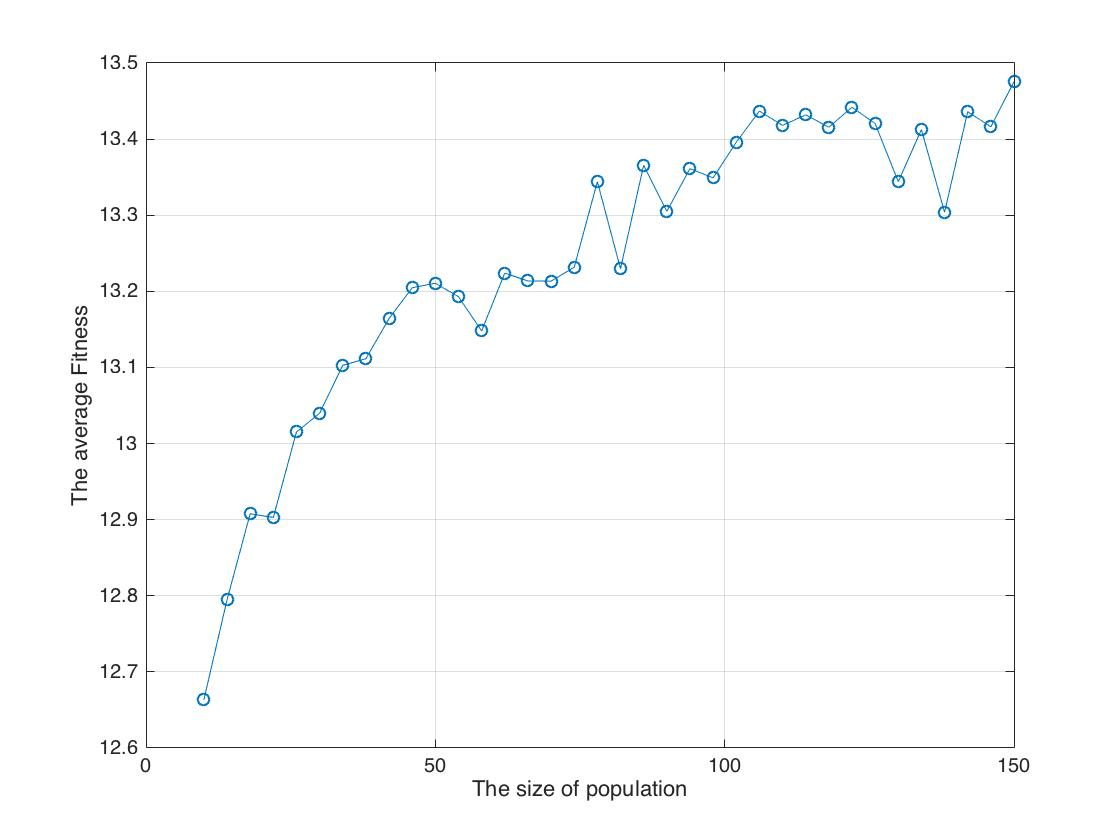
\includegraphics[width=3.5in]{./img/pic5.jpg} 
\label{PS}}
\hfil
\subfloat[Case II]{
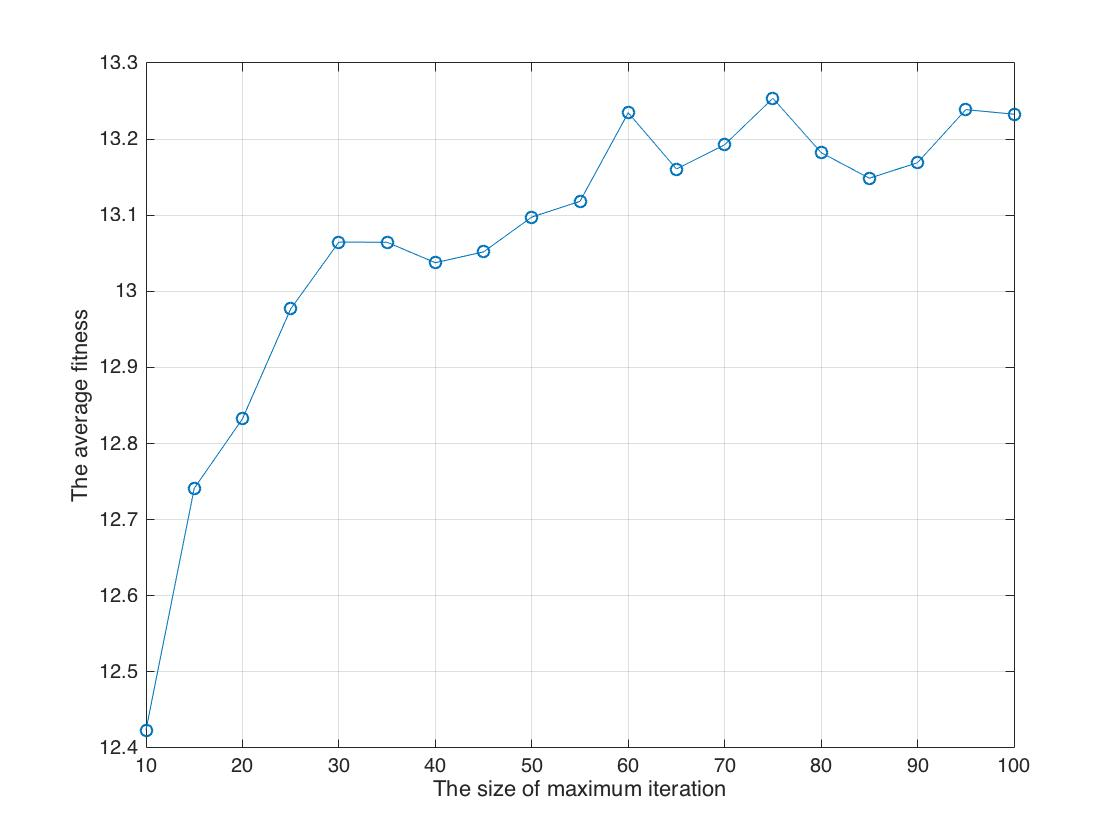
\includegraphics[width=3.5in]{./img/pic6.jpg} 
\label{MI}}

\subfloat[Case III]{
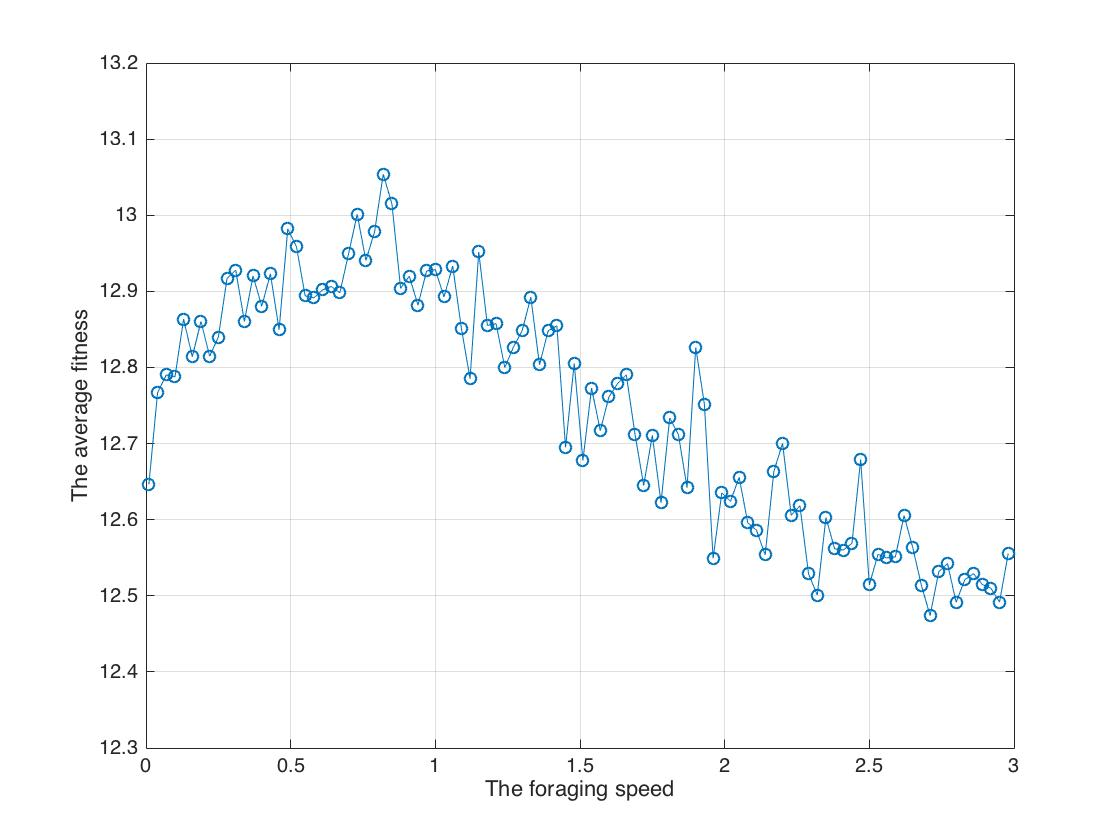
\includegraphics[width=3.5in]{./img/pic7.jpg} 
\label{Vf}}
\hfil
\subfloat[Case IV]{
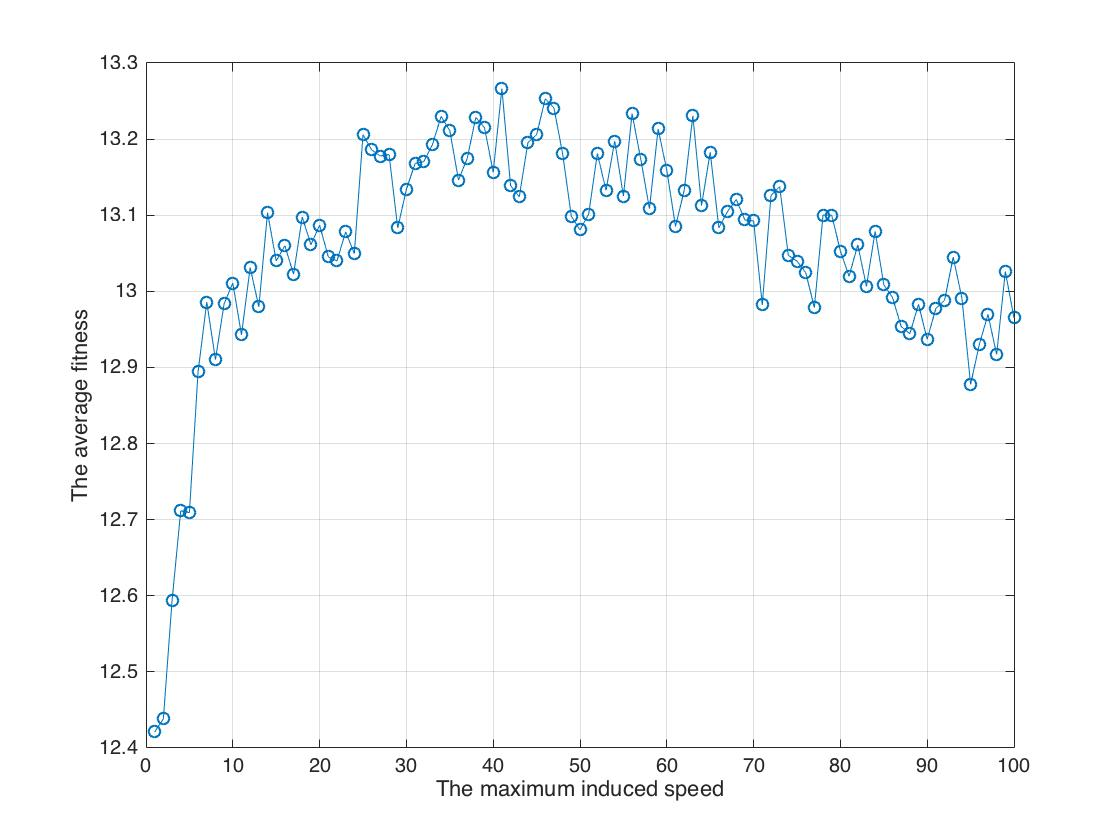
\includegraphics[width=3.5in]{./img/pic8.jpg} 
\label{Nmax}}

\caption{Simulation results for the network.} \label{fig_sim}
\end{figure*}


\subsection{Optimality Evaluation}
To verify the the capability of finding the optimal mobile service composition of our algorithms, we compare KHMSC with the basic GA algorithm, basic PSO algorithm and a brute-force algorithm.

\textit{Algorithm 1:} KH-based mobile service composition algorithm as described in Section 4.

\textit{Algorithm 2:} The normal GA that uses uniform crossover and uniform mutation.

\textit{Algorithm 3:} The normal PSO that uses uniform crossover and uniform mutation.

\textit{Algorithm 4:} A brute-force exhaustive algorithm that traverses all feasible composition to find the optimal solution.

To compare the above algorithms with our approach, we tune the parameters for each algorithm to achieve its best performance. The most suitable parameters are shown in Table III.

\begin{table}[!t]
\renewcommand{\arraystretch}{1.3}
\caption{PARAMETER SETTING OF DIFFERENT ALGORITHMS}
\label{table_example}
\centering
\begin{tabular}{cc}
\hline
\bfseries Algorithms & \bfseries Parameter Setting \\
\hline
GA  & crossover rate = 0.7; mutate rate = 0.3 \\
PSO & ss \\
\hline
\end{tabular}
\end{table}

To evaluate the optimality of the algorithms, we plot the average fitness obtained by all algorithms versus increasing problem size.

The result in Figure 10 shows that, as expected, the brute-force algorithm leads to the best performance with the highest fitness. The basic PSO algorithm has the worst performance with the lowest fitness values. It also shows the highest fluctuations of fitness values because it may easily get trapped by local minima and leads to premature convergence. KHMSC performs better than the basic GA algorithm; it is able to find near optimal composition, mainly because of its knowledge-based crossover and mutation operations.


\subsection{Scalability Evaluation (task number, candidates number)}
In this experiment, we compared the runtime of our algorithms with the other algorithms to evaluate the scalability of our algorithm.

a) Impact of Different Numbers of Tasks
Table V compares the runtime of all algorithms against the number of tasks with a fixed number (100) of services available per task. 
We observe that the runtime of integer programming is nearly hundreds times of KMSCs. 
Since the mobile environment is dynamic, the requirement on runtime must be met because the environment parameters for computation may vary much within a short time. 
Therefore, although integer programming can obtain the optimal result, it is not suitable to the problem in mobile environment due to its poor scalability.
Furthermore, KMSC also runs fastest as compared with the other two population-based algorithms. This is because induced motion, foraging motion, and physical diffusion in KMSC can be executed in parallel, thereby improving the efficiency. Besides, we can observe that KMSC has a low algorithmic complexity, which is roughly linear with the composition size.

b) Impact of Different Numbers of Candidates
Table VI compares the scalability of all algorithms against an increasing number of candidate services with a fixed number (10) of tasks. Similarly, integer programming also performs with the highest runtime. We note that the runtime of all methods is almost irrelevant to the number of services per task. Hence, all algorithms scale well in this regard. Among all the algorithms, KhMSC always performs with the lowest runtime. Based on these results, we can conclude that our approach maintains acceptable performance (optimality and scalability) with large data sets for both tasks and candidates.

\section{RELATED WORK}
Service-oriented computing(SOC) is a novel paradigm to develop and integrate enterprise information system \cite{}, with the development of mobile device and communication technology, the research of mobile service composition has grain much attention from both industry and academia. In this section, we first briefly review some recent work on mobile service composition, then review opportunistic network and its application in mobile network.

\subsection{mobile service composition}
Mobile service computing is the combination of service computing and mobile computing, With the development of mobile device and application industry, more and more study have emerged to address the problem of mobile service composition. 
Deng et al. \cite{Deng2016} presented an detailed introduction to mobile service computing, they first discussed the limitations of mobile computing, then classify mobile service computing into three categories: C2M, M2M, Hybrid. They also discussed the challenge toward mobile service provision and mobile service consumption in terms of performance, energy and security perspective. At their \cite{Deng2017} work, they proposed a mobile service sharing community to address the problem of service provision in mobile environment. They extent the random way point(RWP) model to capture user mobility and utilize the Krill-Herd (KH) algorithm to solve the service composition problem. Yang et al. \cite{Yang2010} presented a comprehensive QoS model specifically for pervasive services. They considered not only mobile wireless network characteristics but also user-perceived factors, and devised a corresponding formula to calculate the QoS criterion. 
zhang et al. \cite{Zhang2016} gives a context-aware service selection algorithm based on Genetic Algorithm to solve the problem of mobile service selection, they introduce a tree-encoding method to improve the capacity and efficiency of GA. However, this work did not consider user mobility.
Wang et al. \cite{wang2011exploiting} solve the problem of dependable service composition in wireless mobile ad hoc networks by taking the mobility prediction of the service providers into consideration.
They use a probability-free model and a probabilistic model to characterize the uncertainty to compose a service that can tolerate the uncertain mobility of service provider. However, this work only focus on the case of sequential service workflows and the heuristic algorithms they presented does not seek the optimal QoS service compositions.

\subsection{mobile opportunistic network}
Opportunistic networking is one of the most interesting evolutions of the multi-hop networking paradigm. Instead of constructing "stable" end-to-end paths as in the Internet, opportunistic networks do not consider node mobility a problem but as an opportunity to exploit. 
Marco et al. \cite{Conti2014} give a review of opportunistic network and regarded it as the first step in people-centric networking, they also discuss the focused research problem such as mobility model and routing problem.
Turkes et al. \cite{turkes2016cocoon} proposed a middleware named Cocoon to support mobile opportunistic network, they design a routing protocol above Wi-Fi and Bluetooth standards, their experiments which use real-world data setups show that Cocoon performs well on the aspects of dissemination rate, delivery latency and energy consumption.
Fortuna et al. \cite{fortuna2009dynamic} presented an review of dynamic service composition over both wired and wireless environment, However, their work does not present any technical details to describe how to composite service in mobile networks.
Giordano et al. \cite{Giordano2011} proposed a novel paradigm that utilize Opportunistic computing as an appealing complement to the mobile computing cloud, in this way, mobile device can combine and exploit heterogeneous resources from other devices.
Pu et al. \cite{Pu2017} presented QoS-oriented self-organized mobile crowdsourcing framework, in this work, the prevalent and sufficient characteristics of opportunistic user encounters in our daily life are utilized to solve crowdsourcing problem.
\section{CONLUSION}

\bibliography{mybibtex}
\bibliographystyle{IEEEtran}

\end{document}






